\RequirePackage[l2tabu, orthodox]{nag}
\RequirePackage{silence}
\WarningFilter{fmtcount}{\ordinal already defined use \FCordinal instead}
\documentclass[english, french]{beamer}
%INSTALL
\pdfgentounicode=1 %permits (with package glyphtounicode) to copy eg x ⪰ y iff v(x) ≥ v(y) from pdf to unicode data. 
\input{glyphtounicode}%TODO avoid warning when redefining → (and others) ; make it work for ℝ (U+211D) as well
\usepackage[T1]{fontenc}%encode resulting accented characters correctly in resulting PDF, permits copy-paste
\usepackage[utf8]{inputenc}
\usepackage{newunicodechar}%able to use e.g. → or ≤ in source
\usepackage{lmodern}%has more characters such as ligatures, permit copy from resulting PDF.
\usepackage{textcomp}%useful for redefining → and ¬ and … (otherwise seems to attempt to use \textrightarrow and the like but are not defined)
% solves bug in lmodern, https://tex.stackexchange.com/a/261188/
\DeclareFontShape{OMX}{cmex}{m}{n}{
  <-7.5> cmex7
  <7.5-8.5> cmex8
  <8.5-9.5> cmex9
  <9.5-> cmex10
}{}

\SetSymbolFont{largesymbols}{normal}{OMX}{cmex}{m}{n}
\SetSymbolFont{largesymbols}{bold}  {OMX}{cmex}{m}{n}
%warn about missing characters
\tracinglostchars=2

%REDAC
\usepackage{booktabs}
\usepackage{calc}
\usepackage{tabularx}

\usepackage{etoolbox} %for addtocmd, newtoggle commands
\newtoggle{LCpres}
\toggletrue{LCpres}

\usepackage{mathtools} %load this before babel!
	\mathtoolsset{showonlyrefs,showmanualtags}

\usepackage{natbib}%Package frenchb asks to load natbib before babel/frenchb
\usepackage{babel}%[french, english]: language options should be on the document level
%suppresses the warning about frenchb not modifying the captions (“—” to “:” in “Figure 1 – Legend”).
%	\frenchbsetup{AutoSpacePunctuation=false,SuppressWarning=true}% test with false?
	\frenchbsetup{AutoSpacePunctuation=false,SuppressWarning=false}

%\usepackage[super]{nth}%better use fmtcount! (loaded by datetime anyway; see below about pbl with warnings and package silence)
\usepackage{listings} %typeset source code listings
	\lstset{language=XML,tabsize=2,captionpos=b,basicstyle=\NoAutoSpacing}%NoAutoSpacing avoids space before colon or ?}%,literate={"}{{\tt"}}1, keywordstyle=\fontspec{Latin Modern Mono Light}\textbf, emph={String, PreparedStatement}, emphstyle=\fontspec{Latin Modern Mono Light}\textbf, language=Java, basicstyle=\small\NoAutoSpacing\ttfamily, frame=single, aboveskip=0pt, belowskip=0pt, showstringspaces=false
\usepackage[nolist,smaller,printonlyused]{acronym}%,smaller option produces warnings from relsize in some cases, it seems.% Note silence and acronym and hyperref make (xe)latex crash when ac used in section (http://tex.stackexchange.com/questions/103483/strange-packages-interaction-acronyms-silence-hyperref), rather use \section{\texorpdfstring{\acs{UE}}{UE}}.
\usepackage{fmtcount}
\usepackage[nodayofweek]{datetime}%must be loaded after the babel package. However, loading it after {nth} generates a warning from fmtcount about ordinal being already defined. Better load it before nth? (then we can remove the silence package which creates possible crashes, see above.) Or remove nth?
%\usepackage{xspace}%do we need this?
\nottoggle{LCpres}{
	\usepackage[textsize=small]{todonotes}
}{
}
\iftoggle{LCpres}{
	%remove pdfusetitle (implied by beamer)
	\usepackage{hyperref}
}{
% option pdfusetitle must be introduced here, not in hypersetup.
	\usepackage[pdfusetitle]{hyperref}
}
\nottoggle{LCpres}{
%seems like authblk wants to be later than hyperref, but sooner than silence
\usepackage{authblk}
\renewcommand\Affilfont{\small}
}{
}
\usepackage{silence}
\WarningFilter{newunicodechar}{Redefining Unicode character}
%breaklinks makes links on multiple lines into different PDF links to the same target.
%colorlinks (false): Colors the text of links and anchors. The colors chosen depend on the the type of link. In spite of colored boxes, the colored text remains when printing.
%linkcolor=black: this leaves other links in colors, e.g. refs in green, don't print well.
%pdfborder (0 0 1, set to 0 0 0 if colorlinks): width of PDF link border
%hidelinks or: colorlinks, linkcolor=black, citecolor=black, urlcolor={blue!80!black}
\hypersetup{breaklinks, bookmarksopen}
%add hyperfigures=true in hypersetup (already defined in article mode)
\iftoggle{LCpres}{
	\hypersetup{hyperfigures}
}{
}

%in Beamer, sets url colored links but does not change the rest of the colors (http://tex.stackexchange.com/questions/13423/how-to-change-the-color-of-href-links-for-real)
%\hypersetup{breaklinks,bookmarksopen,colorlinks=true,urlcolor=blue,linkcolor=,hyperfigures=true}
% hyperref doc says: Package bookmark replaces hyperref’s bookmark organization by a new algorithm (...) Therefore I recommend using this package.
\usepackage{bookmark}

% center floats by default, but do not use with float
% \usepackage{floatrow}
% \makeatletter
% \g@addto@macro\@floatboxreset\centering
% \makeatother
\nottoggle{LCpres}{
	\usepackage{enumitem} %follow enumerate by a string saying how to display enumeration
}{
}
\usepackage{ragged2e} %new com­mands \Cen­ter­ing, \RaggedLeft, and \RaggedRight and new en­vi­ron­ments Cen­ter, FlushLeft, and FlushRight, which set ragged text and are eas­ily con­fig­urable to al­low hy­phen­ation (the cor­re­spond­ing com­mands in LaTeX, all of whose names are lower-case, pre­vent hy­phen­ation al­to­gether). 
\usepackage{siunitx} %[expproduct=tighttimes, decimalsymbol=comma] ou (plus récent ?) [round-mode=figures, round-precision=2, scientific-notation = engineering]
\sisetup{detect-all, locale = FR, strict}% to detect e.g. when in math mode (use a math font) - check whether this makes sense with strict
\usepackage{braket} %for \Set
\usepackage{doi}

\usepackage{amsmath,amsthm}
\usepackage{amssymb}% for \mathbb{R}
\usepackage{bm}%“The \boldsymbol command is obtained preferably by using the bm package, which provides a newer, more powerful version than the one provided by the amsmath package. Generally speaking, it is ill-advised to apply \boldsymbol to more than one symbol at a time.” — AMS Short math guide. “If no bold font appears to be available for a particular symbol, \bm will use ‘poor man’s bold’” — bm
% \usepackage{amsfonts} %not required?
% \usepackage{dsfont} %for what?

\usepackage{environ}%for xdescwd command
%BUT see https://tex.stackexchange.com/questions/83798/cleveref-varioref-missing-endcsname-inserted for cleveref with french
\usepackage{cleveref}% cleveref should go "laster" than hyperref
%GRAPHICS
\usepackage{pgf}
\usepackage{pgfplots}
	\usetikzlibrary{babel, matrix, fit, plotmarks, calc, trees, shapes.geometric, positioning, plothandlers, arrows, shapes.multipart}
\pgfplotsset{compat=1.14}
\usepackage{graphicx}

\DeclareMathAlphabet\mathbfcal{OMS}{cmsy}{b}{n}

\graphicspath{{graphics/},{graphics-dm/}}
\DeclareGraphicsExtensions{.pdf}
\newcommand*{\IncludeGraphicsAux}[2]{%
	\XeTeXLinkBox{%
		\includegraphics#1{#2}%
	}%
}%

%HACKING
\usepackage{printlen}
\uselengthunit{mm}
% 	\newlength{\templ}% or LenTemp?
% 	\setlength{\templ}{6 pt}
% 	\printlength{\templ}
\usepackage{scrhack}% load at end. Corrects a bug in float package, which is outdated but might be used by other packages
\usepackage{mathrsfs}% for \mathscr

%Beamer-specific
%do not remove babel, which beamer uses (beamer uses the \translate command for the appendix); but french can be removed.
\iftoggle{LCpres}{
	\usepackage{appendixnumberbeamer}
	\setbeamertemplate{navigation symbols}{} 
	\usepackage{preamble/beamerthemeParisFrance}
	\usefonttheme{professionalfonts}
	\setcounter{tocdepth}{10}
	%From: http://tex.stackexchange.com/questions/168057/beamer-with-xelatex-on-texlive2013-enumerate-numbers-in-black
%I don’t think it’s useful to submit this as a bug: nothing has been solved since March, 2015. See: https://bitbucket.org/rivanvx/beamer/issues?status=resolved.

\setbeamertemplate{enumerate item}
{
  \begin{pgfpicture}{-1ex}{-0.65ex}{1ex}{1ex}
    \usebeamercolor[fg]{item projected}
    {\pgftransformscale{1.75}\pgftext{\normalsize\pgfuseshading{bigsphere}}}
    {\pgftransformshift{\pgfpoint{0pt}{0.5pt}}
      \pgftext{\usebeamercolor[fg]{item projected}\usebeamerfont*{item projected}\insertenumlabel}}
  \end{pgfpicture}%
}

\setbeamertemplate{enumerate subitem}
{
  \begin{pgfpicture}{-1ex}{-0.55ex}{1ex}{1ex}
    \usebeamercolor[fg]{subitem projected}
    {\pgftransformscale{1.4}\pgftext{\normalsize\pgfuseshading{bigsphere}}}
    \pgftext{%
      \usebeamercolor[fg]{subitem projected}%
      \usebeamerfont*{subitem projected}%
      \insertsubenumlabel}
  \end{pgfpicture}%
}

\setbeamertemplate{enumerate subsubitem}
{
  \begin{pgfpicture}{-1ex}{-0.55ex}{1ex}{1ex}
    \usebeamercolor[fg]{subsubitem projected}
    {\pgftransformscale{1.4}\pgftext{\normalsize\pgfuseshading{bigsphere}}}
    \pgftext{%
      \usebeamercolor[fg]{subsubitem projected}%
      \usebeamerfont*{subitem projected}%
      \insertsubsubenumlabel}
  \end{pgfpicture}%
}


}{
}
% \newcommand{\citep}{\cite}%Better: leave natbib.
% \setbeamersize{text margin left=0.1cm, text margin right=0.1cm} 
% \usetheme{BrusselsBelgium}%no, replace with paris
%\usetheme{ParisFrance}, no, usepackage better!
% Tex Gyre takes too much space, replace with Latin Modern Roman / Sans / Mono.
% Difference when loading explicitly Latin Modern Sans (compared to not using \setsansfont at all):
% the font LMSans17-Regular appears in the document;
% the title of the slides appears differently;
% it does not say (in the log file):
% > LaTeX Font Info:    Font shape `EU1/lmss/m/it' in size <10.95> not available
% > (Font)              Font shape `EU1/lmss/m/sl' tried instead on input line 85.
% > LaTeX Font Info:    Try loading font information for EU1+lmtt on input line 85.

%tikzposter-specific
%remove \usepackage{ragged2e}: causes 1=1 to be printed in the middle of the poster. (Anyway prints a warning about those characters being missing.)
%put [french, english] options next to \usepackage{babel} to avoid warning of 

\NewDocumentCommand{\R}{}{ℝ}
\NewDocumentCommand{\N}{}{ℕ}
%\mathscr is rounder than \mathcal.
\NewDocumentCommand{\powerset}{m}{\mathscr{P}(#1)}
%Powerset without zero.
\NewDocumentCommand{\powersetz}{m}{\mathscr{P}^*(#1)}
%https://tex.stackexchange.com/a/45732, works within both \set and \set*, same spacing than \mid (https://tex.stackexchange.com/a/52905).
\NewDocumentCommand{\suchthat}{}{\;\ifnum\currentgrouptype=16 \middle\fi|\;}
%Integer interval.
\NewDocumentCommand{\intvl}{m}{⟦#1⟧}
%Allows for \abs and \abs*, which resizes the delimiters.
\DeclarePairedDelimiter\abs{\lvert}{\rvert}
\DeclarePairedDelimiter\card{\lvert}{\rvert}
\DeclarePairedDelimiter\floor{\lfloor}{\rfloor}
\DeclarePairedDelimiter\ceil{\lceil}{\rceil}
%Perhaps should use U+2016 ‖ DOUBLE VERTICAL LINE here?
\DeclarePairedDelimiter\norm{\lVert}{\rVert}
%From mathtools. Better than using the package braket because braket introduces possibly undesirable space. Then: \begin{equation}\set*{x \in \R^2 \suchthat \norm{x}<5}\end{equation}.
\DeclarePairedDelimiter\set{\{}{\}}
\DeclareMathOperator*{\argmax}{arg\,max}
\DeclareMathOperator*{\argmin}{arg\,min}

%UTR #25: Unicode support for mathematics recommend to use the straight form of phi (by default, given by \phi) rather than the curly one (by default, given by \varphi), and thus use \phi for the mathematical symbol and not \varphi. I however prefer the curly form because the straight form is too easy to mix up with the symbol for empty set.
\let\phi\varphi

%The amssymb solution.
%\NewDocumentCommand{\restr}{mm}{{#1}_{\restriction #2}}
%Another acceptable solution.
%\NewDocumentCommand{\restr}{mm}{{#1|}_{#2}}
%https://tex.stackexchange.com/a/278631; drawback being that sometimes the text collides with the line below.
\NewDocumentCommand\restr{mm}{#1\raisebox{-.5ex}{$|$}_{#2}}


%Decision Theory (MCDA and SC)
\newcommand{\allalts}{\mathscr{A}}
\newcommand{\allcrits}{\mathscr{C}}
\newcommand{\alts}{A}
\newcommand{\dm}{i}
\newcommand{\allF}{\mathscr{F}}
\newcommand{\allvoters}{\mathscr{N}}
\newcommand{\voters}{N}
\newcommand{\allprofs}{\boldsymbol{\mathcal{R}}}
\newcommand{\prof}{\boldsymbol{R}}
\newcommand{\linors}{\mathscr{L}(\allalts)}
%Thanks to https://tex.stackexchange.com/q/154549
	%\makeatletter
	%\def\@myRgood@#1#2{\mathrel{R^X_{#2}}}
	%\def\myRgood{\@ifnextchar_{\@myRgood@}{\mathrel{R^X}}}
	%\makeatother

%Deliberated Judgment
\newcommand{\allargs}{S^*}
\newcommand{\args}{S}
\newcommand{\ar}{s}
\newcommand{\ileadsto}{⇝}
\newcommand{\ibeatse}{⊳_\exists}
\newcommand{\nibeatse}{⋫_\exists}
\newcommand{\ibeatsst}{⊳_\forall}
\newcommand{\nibeatsst}{⋫_\forall}
\newcommand{\mleadsto}[1][\eta]{⇝_{#1}}
\newcommand{\mbeats}[1][\eta]{⊳_{#1}}
\newcommand{\ibeatseinv}{⊳_\exists^{-1}}

%Logic
\newcommand{\ltru}{\texttt{T}}
\newcommand{\lfal}{\texttt{F}}


%Requires package xcolor.
%\definecolor{ao(english)}{rgb}{0.0, 0.5, 0.0}
\NewDocumentCommand{\commentOC}{m}{\textcolor{blue}{\small$\big[$OC: #1$\big]$}}
%Requires package babel and option [french]. According to babel doc, need two braces around \selectlanguage to make the changes really local.
\NewDocumentCommand{\commentOCf}{m}{\textcolor{blue}{{\small\selectlanguage{french}$\big[$OC : #1$\big]$}}}
\NewDocumentCommand{\commentYM}{m}{\textcolor{red}{\small$\big[$YM: #1$\big]$}}
\NewDocumentCommand{\commentYMf}{m}{\textcolor{red}{{\small\selectlanguage{french}$\big[$YM : #1$\big]$}}}

\bibliographystyle{abbrvnat}
\NewDocumentCommand{\possessivecite}{mO{}}{\citeauthor{#1}’s \citeyearpar[#2]{#1}}

%https://tex.stackexchange.com/a/467188, https://tex.stackexchange.com/a/36088 - uncomment if one of those symbols is used.
%\DeclareFontFamily{U} {MnSymbolD}{}
%\DeclareFontShape{U}{MnSymbolD}{m}{n}{
%  <-6> MnSymbolD5
%  <6-7> MnSymbolD6
%  <7-8> MnSymbolD7
%  <8-9> MnSymbolD8
%  <9-10> MnSymbolD9
%  <10-12> MnSymbolD10
%  <12-> MnSymbolD12}{}
%\DeclareFontShape{U}{MnSymbolD}{b}{n}{
%  <-6> MnSymbolD-Bold5
%  <6-7> MnSymbolD-Bold6
%  <7-8> MnSymbolD-Bold7
%  <8-9> MnSymbolD-Bold8
%  <9-10> MnSymbolD-Bold9
%  <10-12> MnSymbolD-Bold10
%  <12-> MnSymbolD-Bold12}{}
%\DeclareSymbolFont{MnSyD} {U} {MnSymbolD}{m}{n}
%\DeclareMathSymbol{\ntriplesim}{\mathrel}{MnSyD}{126}
%\DeclareMathSymbol{\nlessgtr}{\mathrel}{MnSyD}{192}
%\DeclareMathSymbol{\ngtrless}{\mathrel}{MnSyD}{193}
%\DeclareMathSymbol{\nlesseqgtr}{\mathrel}{MnSyD}{194}
%\DeclareMathSymbol{\ngtreqless}{\mathrel}{MnSyD}{195}
%\DeclareMathSymbol{\nlesseqgtrslant}{\mathrel}{MnSyD}{198}
%\DeclareMathSymbol{\ngtreqlessslant}{\mathrel}{MnSyD}{199}
%\DeclareMathSymbol{\npreccurlyeq}{\mathrel}{MnSyD}{228}
%\DeclareMathSymbol{\nsucccurlyeq}{\mathrel}{MnSyD}{229}
%\DeclareFontFamily{U} {MnSymbolA}{}
%\DeclareFontShape{U}{MnSymbolA}{m}{n}{
%  <-6> MnSymbolA5
%  <6-7> MnSymbolA6
%  <7-8> MnSymbolA7
%  <8-9> MnSymbolA8
%  <9-10> MnSymbolA9
%  <10-12> MnSymbolA10
%  <12-> MnSymbolA12}{}
%\DeclareFontShape{U}{MnSymbolA}{b}{n}{
%  <-6> MnSymbolA-Bold5
%  <6-7> MnSymbolA-Bold6
%  <7-8> MnSymbolA-Bold7
%  <8-9> MnSymbolA-Bold8
%  <9-10> MnSymbolA-Bold9
%  <10-12> MnSymbolA-Bold10
%  <12-> MnSymbolA-Bold12}{}
%\DeclareSymbolFont{MnSyA} {U} {MnSymbolA}{m}{n}
%%Rightwards wave arrow: ↝. Alternative: \rightsquigarrow from amssymb, but it’s uglier
%\DeclareMathSymbol{\rightlsquigarrow}{\mathrel}{MnSyA}{160}

%03B3 Greek Small Letter Gamma
\newunicodechar{γ}{\gamma}
%03B4 Greek Small Letter Delta
\newunicodechar{δ}{\delta}
%2115 Double-Struck Capital N
\newunicodechar{ℕ}{\mathbb{N}}
%211D Double-Struck Capital R
\newunicodechar{ℝ}{\mathbb{R}}
%21CF Rightwards Double Arrow with Stroke
\newunicodechar{⇏}{\nRightarrow}
%21D2 Rightwards Double Arrow
\newunicodechar{⇒}{\ensuremath{\Rightarrow}}
%21D4 Left Right Double Arrow
\newunicodechar{⇔}{\Leftrightarrow}
%21DD Rightwards Squiggle Arrow
\newunicodechar{⇝}{\rightsquigarrow}
%2205 Empty Set
\newunicodechar{∅}{\emptyset}
%2212 Minus Sign
\newunicodechar{−}{\ifmmode{-}\else\textminus\fi}
%2227 Logical And
\newunicodechar{∧}{\land}
%2228 Logical Or
\newunicodechar{∨}{\lor}
%2229 Intersection
\newunicodechar{∩}{\cap}
%222A Union
\newunicodechar{∪}{\cup}
%2260 Not Equal To (handy also as text in informal writing)
\newunicodechar{≠}{\ensuremath{\neq}}
%2264 Less-Than or Equal To
\newunicodechar{≤}{\leq}
%2265 Greater-Than or Equal To
\newunicodechar{≥}{\geq}
%2270 Neither Less-Than nor Equal To
\newunicodechar{≰}{\nleq}
%2271 Neither Greater-Than nor Equal To
\newunicodechar{≱}{\ngeq}
%2272 Less-Than or Equivalent To
\newunicodechar{≲}{\lesssim}
%2273 Greater-Than or Equivalent To
\newunicodechar{≳}{\gtrsim}
%2274 Neither Less-Than nor Equivalent To – also, from MnSymbol: \nprecsim, a more exact match to the Unicode symbol; and \npreccurlyeq, too small
\newunicodechar{≴}{\not\preccurlyeq}
%2275 Neither Greater-Than nor Equivalent To
\newunicodechar{≵}{\not\succcurlyeq}
%2279 Neither Greater-Than nor Less-Than – requires MnSymbol; also \nlessgtr from txfonts/pxfonts, \ngtreqless from MnSymbol (but much higher), \ngtrless from MnSymbol (a more exact match to the Unicode symbol); for incomparability (not matching this Unicode symbol), may also consider \ntriplesim from MnSymbol,\nparallelslant from fourier, \between from mathabx, or ⋈
\newunicodechar{≹}{\ngtreqlessslant}
%227A Precedes
\newunicodechar{≺}{\prec}
%227B Succeeds
\newunicodechar{≻}{\succ}
%227C Precedes or Equal To
\newunicodechar{≼}{\preccurlyeq}
%227D Succeeds or Equal To
\newunicodechar{≽}{\succcurlyeq}
%227E Precedes or Equivalent To
\newunicodechar{≾}{\precsim}
%227F Succeeds or Equivalent To
\newunicodechar{≿}{\succsim}
%2280 Does Not Precede
\newunicodechar{⊀}{\nprec}
%2281 Does Not Succeed
\newunicodechar{⊁}{\nsucc}
%2286
\newunicodechar{⊆}{\subseteq}
%22B2 Normal Subgroup Of – using \vartriangleleft from amsfonts, which goes well with \trianglelefteq, \ntriangleright, and so on, also from amsfonts; another possibility is \lhd from latexsym, which seems visually equivalent to \vartriangleleft from amsfonts; latexsym also has ⊴=\unlhd, but doesn’t have a symbol for ⊴. Other related symbols: \triangleleft from latesym package is too small; fdsymbol provides \triangleleft=\medtriangleleft and \vartriangleleft=\smalltriangleleft; MnSymbol provides \medtriangleleft and \vartriangleleft=\lessclosed=\lhd which are smaller than \vartriangleleft from amsfont; \vartriangleleft from mathabx (p. 67), looks different (wider); also \vartriangleleft from boisik (p. 69) looks still different; \vartriangleleft=\lhd from stix are smaller. Oddly enough, \triangleright appears as the LMMathItalic12-Regular font whereas \rhd appears as LASY10 and \vartriangleright appears as MSAM10.
\newunicodechar{⊲}{\vartriangleleft}
%22B3 Contains as Normal Subgroup (also: 25B7 White right-pointing triangle or 25B9 White right-pointing small triangle)
\newunicodechar{⊳}{\vartriangleright}
%22B4 Normal Subgroup of or Equal To
\newunicodechar{⊴}{\trianglelefteq}
%22B5 Contains as Normal Subgroup or Equal To
\newunicodechar{⊵}{\trianglerighteq}
%22C8 Bowtie
\newunicodechar{⋈}{\bowtie}
%22EA Not Normal Subgroup Of
\newunicodechar{⋪}{\ntriangleleft}
%22EB Does Not Contain As Normal Subgroup
\newunicodechar{⋫}{\ntriangleright}
%22EC Not Normal Subgroup of or Equal To
\newunicodechar{⋬}{\ntrianglelefteq}
%22ED Does Not Contain as Normal Subgroup or Equal
\newunicodechar{⋭}{\ntrianglerighteq}
%25A1 White Square
\newunicodechar{□}{\Box}
%27E6 Mathematical Left White Square Bracket – requires stmaryrd (alternative: \text{\textlbrackdbl}, but ugly if used in an italicized text such as a theorem)
\newunicodechar{⟦}{\llbracket}
%27E7 Mathematical Right White Square Bracket
\newunicodechar{⟧}{\rrbracket}
%27FC Long Rightwards Arrow from Bar
\newunicodechar{⟼}{\longmapsto}
%2AB0 Succeeds Above Single-Line Equals Sign
\newunicodechar{⪰}{\succeq}
%301A Left White Square Bracket
\newunicodechar{〚}{\textlbrackdbl}
%301B Right White Square Bracket
\newunicodechar{〛}{\textrbrackdbl}
%→ is defined by default as \textrightarrow, which is invalid in math mode. Same thing for the three other commands. Using \DeclareUnicodeCharacter instead of \newunicodechar because the latter warns about the previous definition.
%← Leftwards Arrow
\DeclareUnicodeCharacter{2190}{\ifmmode\leftarrow\else\textleftarrow\fi}
%→ Rightwards Arrow
\DeclareUnicodeCharacter{2192}{\ifmmode\rightarrow\else\textrightarrow\fi}
%¬ Not Sign
\DeclareUnicodeCharacter{00AC}{\ifmmode\lnot\else\textlnot\fi}
%… Horizontal Ellipsis
\DeclareUnicodeCharacter{2026}{\ifmmode\dots\else\textellipsis\fi}
%× Multiplication Sign
\DeclareUnicodeCharacter{00D7}{\ifmmode\times\else\texttimes\fi}
%Permits to really obtain a straight quote when typing a straight quote; potentially dangerous, see https://tex.stackexchange.com/a/521999
\catcode`\'=\active
\DeclareUnicodeCharacter{0027}{\ifmmode^\prime\else\textquotesingle\fi}

\newcommand{\mkkOK}{\checkmark}%\color{green}{\checkmark}
\newcommand{\mkkREQ}{\ding{53}}%requires pifont?%\color{green}{\checkmark}
\newcommand{\mkkNO}{\color{red}{\textsf{X}}}


\NewDocumentCommand{\tikzmark}{m}{%
	\tikz[overlay, remember picture, baseline=(#1.base)] \node (#1) {};%
}

\newlength{\GraphsDNodeSep}
\setlength{\GraphsDNodeSep}{7mm}
\tikzset{/GraphsD/dot/.style={
	shape=circle, fill=black, inner sep=0, minimum size=1mm
}}

% MCDA Drawing Sorting
\newlength{\MCDSCatHeight}
\setlength{\MCDSCatHeight}{6mm}
\newlength{\MCDSAltHeight}
\setlength{\MCDSAltHeight}{4mm}
%separation between two vertical alts
\newlength{\MCDSAltSep}
\setlength{\MCDSAltSep}{2mm}
\newlength{\MCDSCatWidth}
\setlength{\MCDSCatWidth}{3cm}
\newlength{\MCDSAltWidth}
\setlength{\MCDSAltWidth}{2.5cm}
\newlength{\MCDSEvalRowHeight}
\setlength{\MCDSEvalRowHeight}{6mm}
\newlength{\MCDSAltsToCatsSep}
\setlength{\MCDSAltsToCatsSep}{1.5cm}
\newcounter{MCDSNbAlts}
\newcounter{MCDSNbCats}
\newlength{\MCDSArrowDownOffset}
\setlength{\MCDSArrowDownOffset}{0mm}
\tikzset{/MCD/S/alt/.style={
	shape=rectangle, draw=black, inner sep=0, minimum height=\MCDSAltHeight, minimum width=\MCDSAltWidth
}}
\tikzset{/MCD/S/pref/.style={
	shape=ellipse, draw=gray, thick
}}
\tikzset{/MCD/S/cat/.style={
	shape=rectangle, draw=black, inner sep=0, minimum height=\MCDSCatHeight, minimum width=\MCDSCatWidth
}}
\tikzset{/MCD/S/evals matrix/.style={
	matrix, row sep=-\pgflinewidth, column sep=-\pgflinewidth, nodes={shape=rectangle, draw=black, inner sep=0mm, text depth=0.5ex, text height=1em, minimum height=\MCDSEvalRowHeight, minimum width=12mm}, nodes in empty cells, matrix of nodes, inner sep=0mm, outer sep=0mm, row 1/.style={nodes={draw=none, minimum height=0em, text height=, inner ysep=1mm}}
}}

%Git
\newlength{\GitDCommitSep}
\setlength{\GitDCommitSep}{13mm}
\tikzset{/GitD/commit/.style={
	shape=rectangle, draw, minimum width=4em, minimum height=0.6cm
}}
\tikzset{/GitD/branch/.style={
	shape=ellipse, draw, red
}}
\tikzset{/GitD/head/.style={
	shape=ellipse, draw, fill=yellow
}}

%Social Choice
\tikzset{/SCD/profile matrix/.style={
	matrix of math nodes, column sep=3mm, row sep=2mm, nodes={inner sep=0.5mm, anchor=base}
}}
\tikzset{/SCD/rank-profile matrix/.style={
	matrix of math nodes, column sep=3mm, row sep=2mm, nodes={anchor=base}, column 1/.style={nodes={inner sep=0.5mm}}, row 1/.style={nodes={inner sep=0.5mm}}
}}
\tikzset{/SCD/rank-vector/.style={
	draw, rectangle, inner sep=0, outer sep=1mm
}}
\tikzset{/SCD/isolated rank-vector/.style={
	draw, matrix of math nodes, column sep=3mm, inner sep=0, matrix anchor=base, nodes={anchor=base, inner sep=.33em}, ampersand replacement=\&
}}

% GUI
\tikzset{/GUID/button/.style={
	rectangle, very thick, rounded corners, draw=black, fill=black!40%, top color=black!70, bottom color=white
}}

% Logger objects
\tikzset{/loggerD/main/.style={
	shape=rectangle, draw=black, inner sep=1ex, minimum height=7mm
}}
\tikzset{/loggerD/helper/.style={
	shape=rectangle, draw=black, dashed, minimum height=7mm
}}
\tikzset{/loggerD/helper line/.style={
	<->, draw, dotted
}}

% Beliefs
\tikzset{/BeliefsD/attacker/.style={
	shape=rectangle, draw, minimum size=8mm
}}
\tikzset{/BeliefsD/supporter/.style={
	shape=circle, draw
}}


\DeclareAcronym{AMCD}{short=amcd, long={Aide Multicritère à la Décision}}
\DeclareAcronym{AR}{short=ar, long={Argumentative Recommender}}
\DeclareAcronym{DA}{short=da, long={Decision Analysis}}
\DeclareAcronym{DJ}{short=dj, long={Deliberated Judgment}}
\DeclareAcronym{DM}{short=dm, long={Decision Maker}}
\DeclareAcronym{DP}{short=dp, long={Deliberated Preference}}
\DeclareAcronym{MAVT}{short=mavt, long={Multiple Attribute Value Theory}}
\DeclareAcronym{MCDA}{short=mcda, long={Multicriteria Decision Aid}}
\DeclareAcronym{MIP}{short=mip, long={Mixed Integer Program}}


%this approach does not generalize to multipart nodes.
%\tikzset{/uml/interface/.style={rectangle, draw, fill=yellow!20, align=left, node font=\fontspec{Latin Modern Mono Light}, node contents={$<<$interface$>>$\\\textbf{#1}}, name=#1
%}}
%this approach does not apply for <<interface>>. Never mind, I’ll do it manually, as I can’t find anything better. Use: \nodepart[font=]{one} \small <<interface>>\\\bfseries ItemDAO
\tikzset{/uml/class/.style={rectangle, draw, align=center, fill=yellow!20, node font=\fontspec{Latin Modern Mono Light}, font=\bfseries
}}
\tikzset{/uml/abstract class/.style={rectangle, draw, align=center, fill=yellow!20, node font=\fontspec{Latin Modern Mono Light}, font=\bfseries\itshape
}}
\tikzset{/uml/class3/.style={
rectangle split, rectangle split every empty part={}, rectangle split parts=3, rectangle split part align={center, left, left}, draw, fill=yellow!20, rectangle split empty part height=0, node font=\fontspec{Latin Modern Mono Light}, every one node part/.style={font=\bfseries, align=center}, every two node part/.style={align=left}, every three node part/.style={align=left}
}}
\tikzset{/uml/extends/.style={draw, -open triangle 45}}
\tikzset{/uml/implements/.style={draw, -open triangle 45, dashed}}
%prefix= used to cancel \texttt, otherwise this cancels the effect of the font selection \fontspec{Latin Modern Mono Light}, and thus renders \bfseries inoperant. With prefix=, the result is correct.
%\jeeref[prefix=]{javax.faces.component.html/HtmlCommandButton}\\
\tikzset{/uml/table/.style={rectangle, draw, align=center, fill=blue!20, node font=\fontspec{Latin Modern Mono Light}, font=\bfseries
}}
\tikzset{/uml/table2/.style={
rectangle split, rectangle split every empty part={}, rectangle split parts=2, rectangle split part align={center, left}, draw, fill=blue!20, rectangle split empty part height=0, node font=\fontspec{Latin Modern Mono Light}, every one node part/.style={font=\bfseries, align=center}, every two node part/.style={align=left}
}}
\tikzset{/uml/dbkey/.style={draw, ->}}
%http://tex.stackexchange.com/questions/79781/placing-anchor-before-and-after-text-in-multipart-rectangle



\setbeamertemplate{headline}[singleline]
\setbeamertemplate{footline}[onlypage]

\title{Conception d’applications web en Java}
\subtitle{Présentation du cours}
\author{Olivier Cailloux}
\institute[LAMSADE]{LAMSADE, Université Paris-Dauphine}
\date{Version du \today}

\begin{document}
\bibliographystyle{apalike}

\begin{frame}[plain]
	\tikz[remember picture,overlay]{
		\path (current page.south west) node[anchor=south west, inner sep=0] {
			
\includegraphics[height=1cm]{LAMSADE95.jpg}
		};
		\path (current page.south) ++ (0, 1mm) node[anchor=south, inner sep=0] {
			
\includegraphics[height=9mm]{Dauphine.jpg}
		};
		\path (current page.south east) node[anchor=south east, inner sep=0] {
			
\includegraphics[height=1cm]{PSL.png}
		};
	}
   \titlepage
\end{frame}
\addtocounter{framenumber}{-1}

\section{L’enseignant}
\begin{frame}
	\frametitle{L’enseignant}
	\begin{itemize}
		\item Olivier Cailloux
		\item \href{mailto:olivier.cailloux@dauphine.fr}{olivier.cailloux@dauphine.fr}
		\item Coordonnées : cf. \href{https://www.ent.dauphine.fr/annuaire/index.php?param0=fiche&param1=ocailloux}{annuaire} de Dauphine
	\end{itemize}
\end{frame}

\section[Obj. pédagogiques]{Objectifs pédagogiques}
\subsection{Objectifs pédagogiques}
\begin{frame}
	\frametitle{Objectifs pédagogiques}
	\begin{itemize}
		\item Programmer des applications d’envergure
		\item De qualité
		\item Portables
		\begin{itemize}
			\item Appui sur API ouvertes
			\item Programmer selon les specs
		\end{itemize}
		\item Programmation Java (mais surtout principes généraux !)
	\end{itemize}
\end{frame}

\begin{frame}
	\frametitle{Objectifs pédagogiques (plus précisément)}
	\begin{block}{Architecture web}
		Appui sur quelques standards du web actuels
		\begin{itemize}
			\item Services Web REST
			\item Formats complémentaires : XML et JSON
			\item BD SQL et ORM
			\item Réduction de la complexité par division
		\end{itemize}
	\end{block}
	\begin{itemize}
		\item Prise en main d’outils de dév avancés : 
		\begin{itemize}
			\item Eclipse ;
			\item Maven ;
			\item Git…
		\end{itemize}
		\item Beaucoup de paramètres ⇒ comprendre !
	\end{itemize}
\end{frame}

\begin{frame}
	\frametitle{Objectifs pédagogiques (agilité)}
	Approche agile ? En partie !
	\begin{itemize}
		\item Livraisons fréquentes
		\item Réusinage fréquent
	\end{itemize}
\end{frame}

\subsection{Obligation de comprendre}
\begin{frame}[fragile]
	\frametitle{Un environnement imparfait}
	\begin{minipage}{\columnwidth+15mm}
	\hspace{-8mm}%
	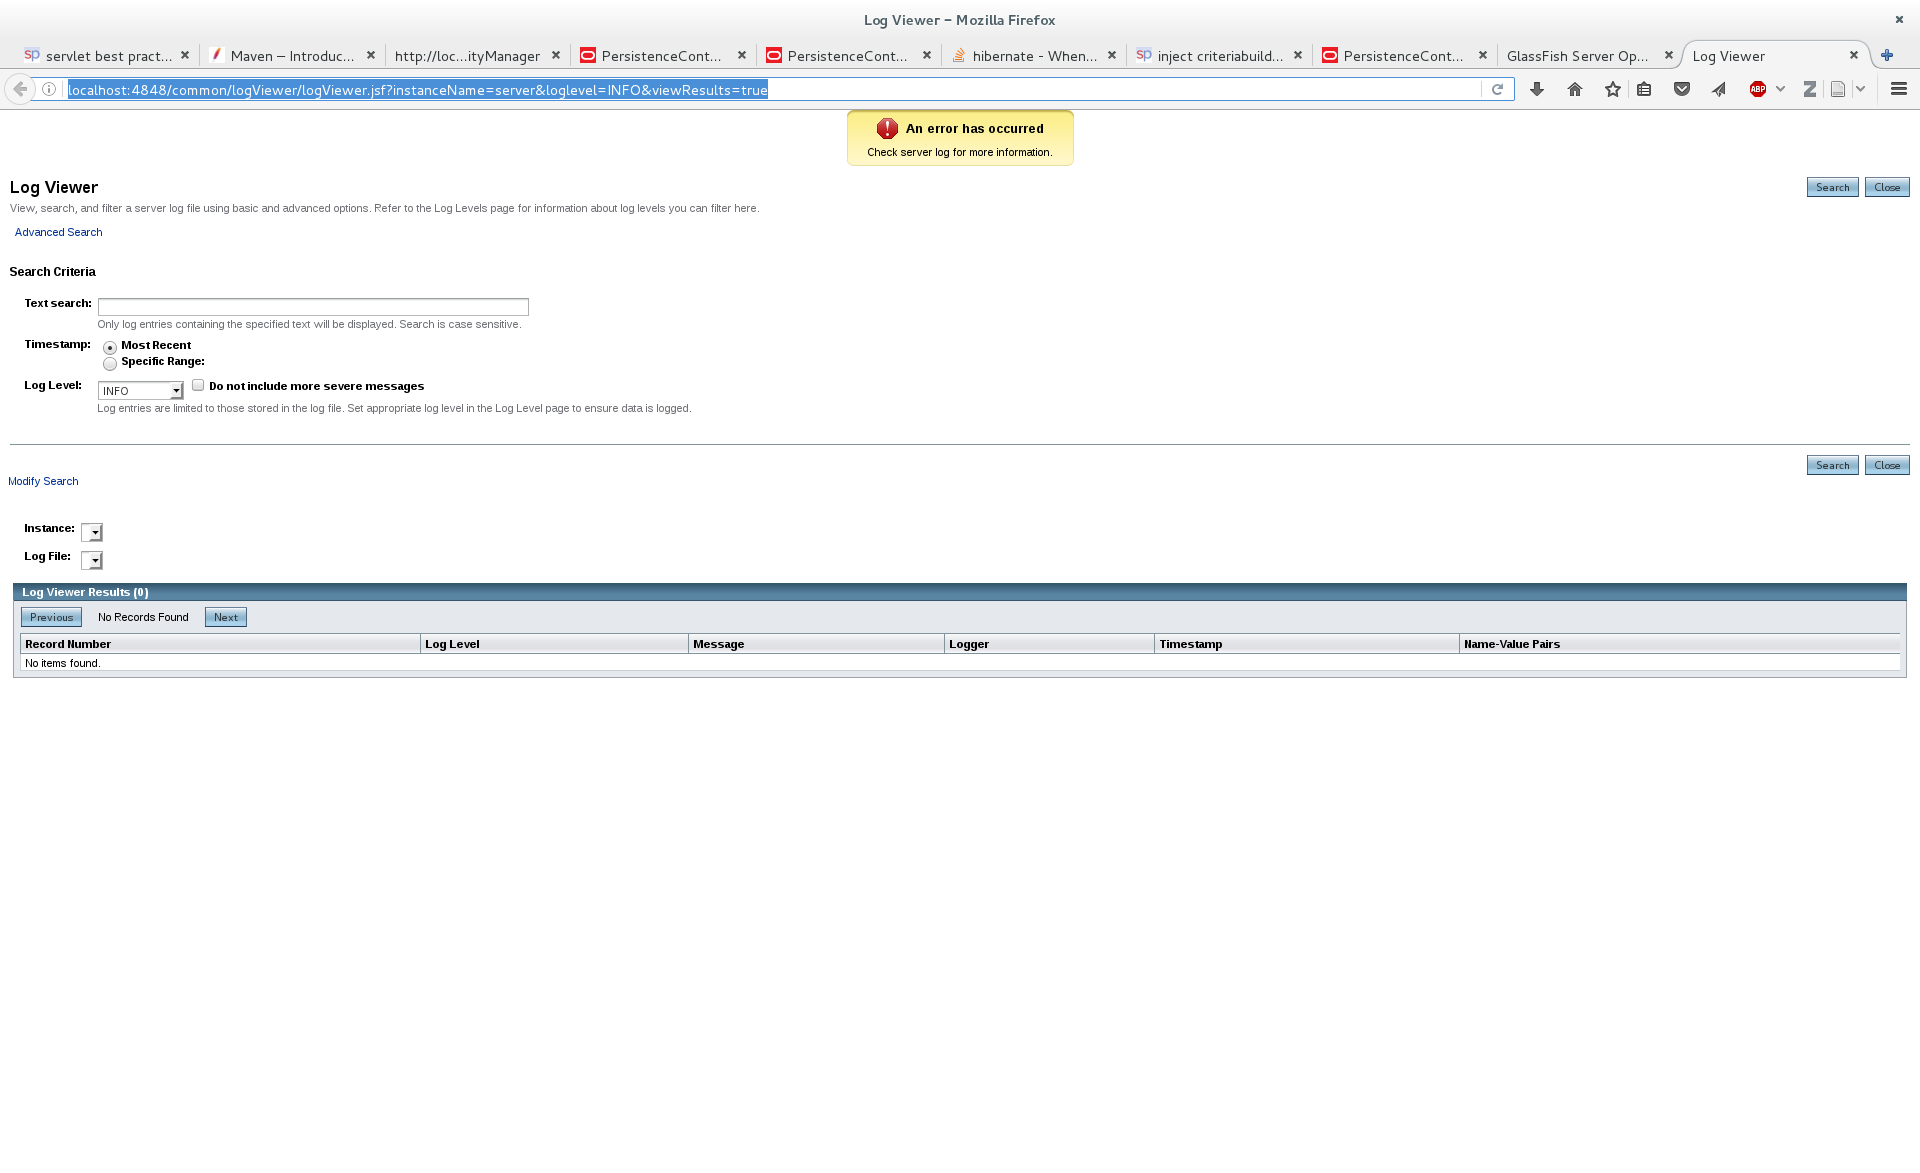
\includegraphics[width=\columnwidth, trim = 0 20cm 28cm 0, clip]{Check_log.png}%
	\end{minipage}
\end{frame}

\begin{frame}
	\frametitle{Un environnement complexe}
	De \url{http://graphserver.github.io/graphserver/} :
	\begin{quote}
		First, get Java 1.6. Or Java6. I think they're the same thing. Get the JDK, but not the JVM, the JRE, SDK, SDN, or the JCE. Note Java SE comes with Jave EE, which is apparently at version 5, and may or may not have anything to do with J2EE. I don't know what those have to do with anything. Google it or something. I don't know. They don't make it particularly easy for you. It's like, they've got more money than god and nothing pleases them better than pouring all that expertise into baffling the hell out of you. Honestly, I can't stand Java, but you need it to run Osmosis.
	\end{quote}
\end{frame}

\subsection{Utilité}
\begin{frame}
	\frametitle{Intérêt pratique}
	\begin{itemize}
		\item Qu’on soit programmeur, qu’on discute avec des programmeurs
		\item Prendre de la hauteur, éviter les tâches répétitives et se concentrer sur le conceptuel
		\item Respect et compréhension des standards (aperçu de la façon dont ils sont construits) : compétence essentielle
		\item … dans de multiples domaines
		\item Technologie en vogue
		\begin{itemize}
			\item Java EE VS Spring VS … ?
		\end{itemize}
	\end{itemize}
\end{frame}

\begin{frame}
	\frametitle{Les bienfaits de la complexité}
	\begin{minipage}{6cm}
		\begin{itemize}
			\item Activité plus difficile : souvent plus attrayante
			\item Évite les activités répétitives : complexité amène diversité
			\item Récompenses plus grandes
			\item Recherche d’un accomplissement personnel
			\item Cercle vertueux : accès à activités plus complexes
			\item Pas un bien positionnel : accessible à tous
		\end{itemize}
	\end{minipage}\hspace{5mm}%
	\begin{minipage}{\columnwidth-6.5cm}
		\href{https://fr.wikipedia.org/wiki/\%C3\%89criture_hi\%C3\%A9ratique}{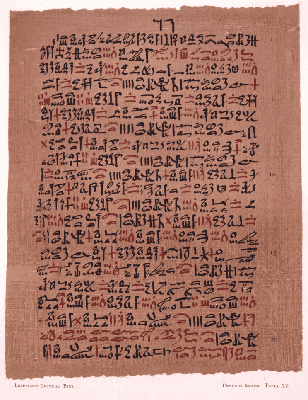
\includegraphics[width=\columnwidth]{Papyrus_Ebers.png}}
		\small{Écriture \href{https://en.wikipedia.org/wiki/Hieratic}{hiératique}, égypte ancienne}
	\end{minipage}
\end{frame}

\subsection{Prérequis}
\begin{frame}
	\frametitle{Prérequis}
	\begin{itemize}
		\item Programmation en Java, manipulation d’un environnement de développement, compréhension des notions algorithmiques élémentaires.
		\item Capacité à comprendre des textes en anglais liés à l’informatique.
		\item HTTP, HTML, XML, SQL.
	\end{itemize}
\end{frame}

\section{Mise en œuvre}
\subsection{Mise en œuvre}
\begin{frame}
	\frametitle{Mise en œuvre}
	\begin{itemize}
		\item Central : travail sur projet
		\item Objectif : un projet utile
		\item Un projet ≠ par groupe
		\item Travail par fonctionnalité
		\item Livraisons exclusivement via git
	\end{itemize}
\end{frame}

	\newlength{\agTotHeight}
	\newlength{\agTotWidth}
	\settoheight{\agTotHeight}{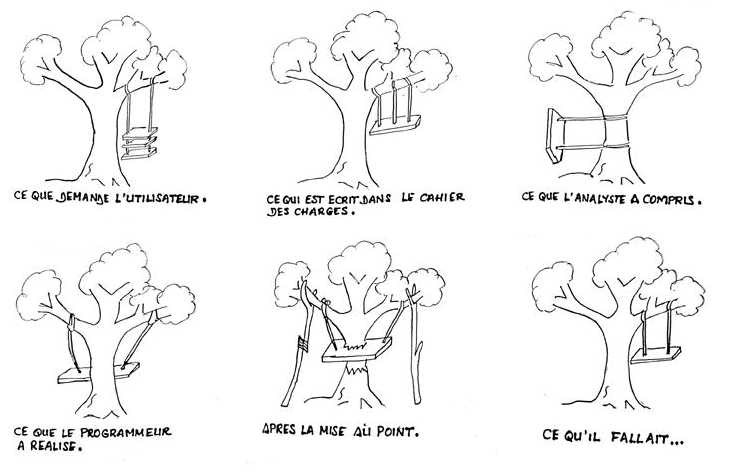
\includegraphics{Demarcheinformatique.jpg}}
	\settowidth{\agTotWidth}{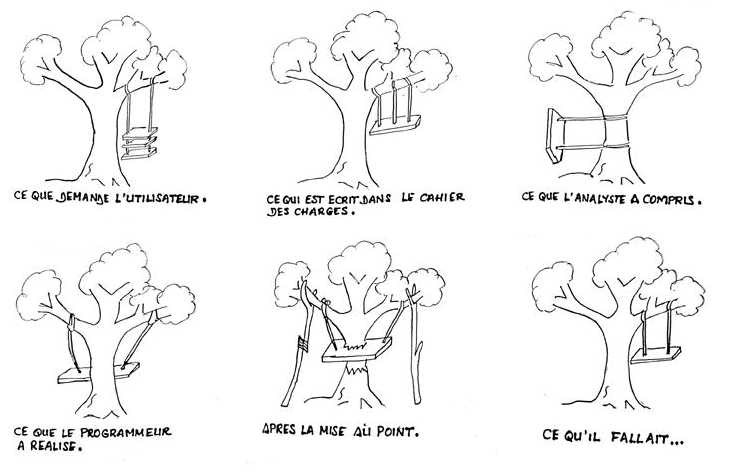
\includegraphics{Demarcheinformatique.jpg}}
	\newlength{\agTopHalf}
	\setlength{\agTopHalf}{\agTotHeight / 2 + 1mm}
	\newlength{\agBottomHalf}
	\setlength{\agBottomHalf}{\agTotHeight / 2 + 1mm}
	\newlength{\agPanelWidth}
	\setlength{\agPanelWidth}{\agTotWidth / 3}
	\newlength{\agWidth}
	\setlength{\agWidth}{3.0cm - 1pt}
	\newlength{\agTopCrop}
	\setlength{\agTopCrop}{3mm}
	\newlength{\agBottomCrop}
	\setlength{\agBottomCrop}{6mm}
\begin{frame}
	\frametitle{Agilité}
	\begin{itemize}
		\item Je joue le rôle du client : détail des fonctionnalités à implémenter
		\item Fonctionnalités de l’application décrites de manière vague : à vous de m’interroger
	\end{itemize}
	\begin{center}
		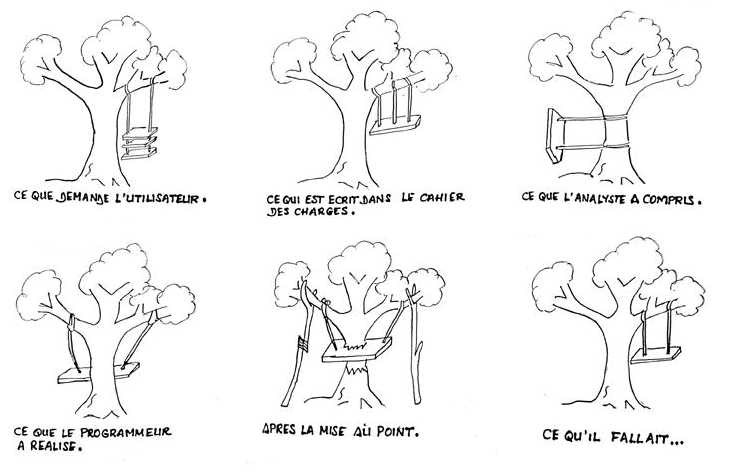
\includegraphics[clip, trim=0 \agBottomHalf{} 2\agPanelWidth{} \agTopCrop{}, width=\agWidth]{Demarcheinformatique.jpg}%
		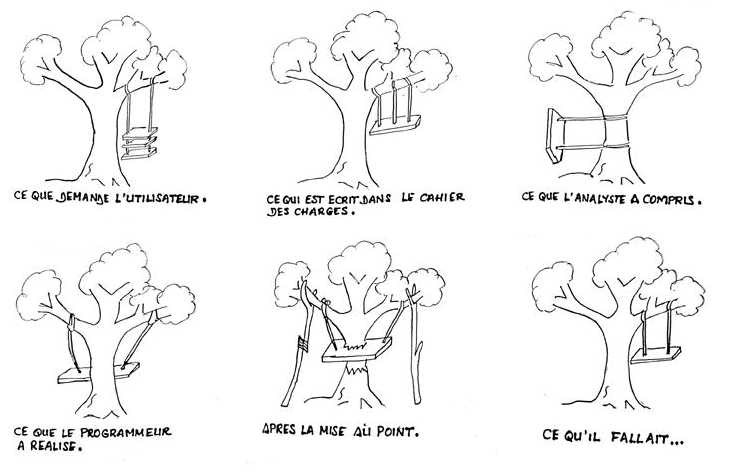
\includegraphics[clip, trim=\agPanelWidth{} \agBottomHalf{} \agPanelWidth{} \agTopCrop{}, width=\agWidth]{Demarcheinformatique.jpg}%
		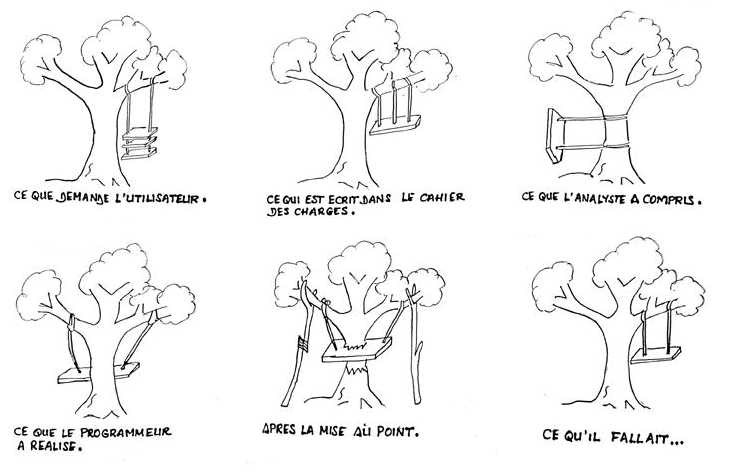
\includegraphics[clip, trim=2\agPanelWidth{} \agBottomHalf{} 0 \agTopCrop{}, width=\agWidth]{Demarcheinformatique.jpg}%
			
		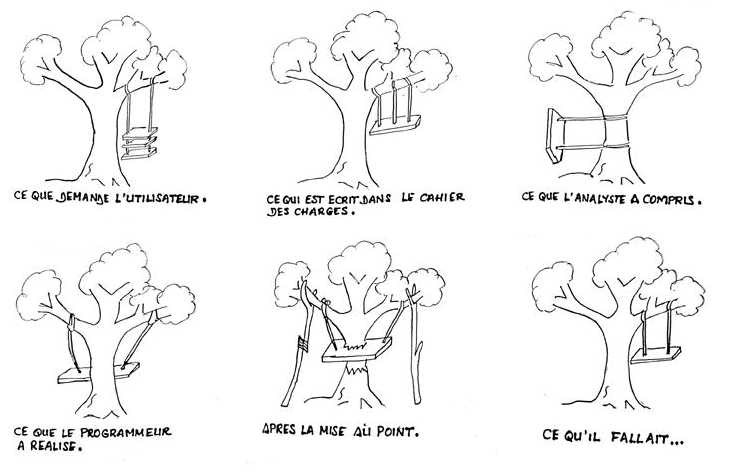
\includegraphics[clip, trim=0 \agBottomCrop{} 2\agPanelWidth{} \agTopHalf{}, width=\agWidth]{Demarcheinformatique.jpg}%
		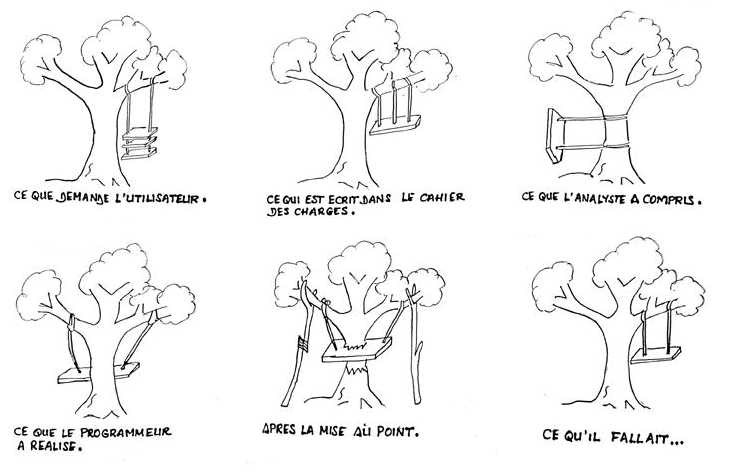
\includegraphics[clip, trim=\agPanelWidth{} \agBottomCrop{} \agPanelWidth{} \agTopHalf{}, width=\agWidth]{Demarcheinformatique.jpg}%
		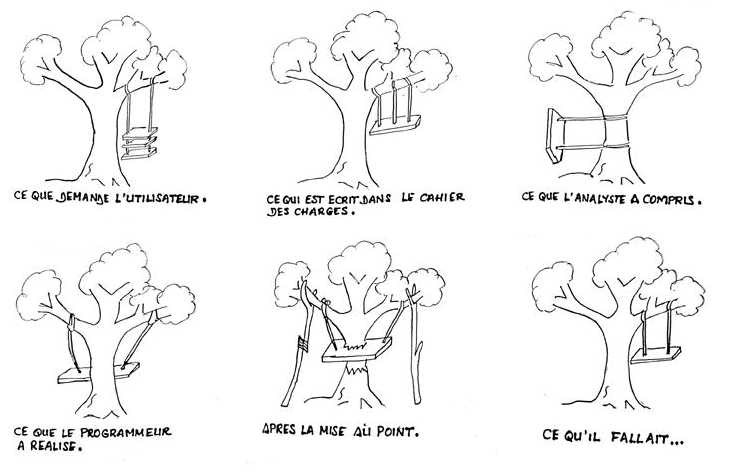
\includegraphics[clip, trim=2\agPanelWidth{} \agBottomCrop{} 0 \agTopHalf{}, width=\agWidth]{Demarcheinformatique.jpg}%
	\end{center}
\end{frame}

\subsection{Évaluation}
\begin{frame}
	\frametitle{Évaluation}
	 Évaluation individuelle et collective !
	\begin{itemize}
		\item 50\% CC
		\begin{itemize}
			\item Devoirs et travaux en séance (via GitHub Classroom)
		\end{itemize}
		\item 50\% Projet (fin d’année)
		\begin{itemize}
			\item Points de difficultés reçus pour fonctionnalité quand qualité atteinte
			\item Trois points de difficultés exigés sur l’année
			\item Présentation collective de vos projets
		\end{itemize}
		\item Fin d’année : Vote pour la meilleure application
	\end{itemize}
\end{frame}

\begin{frame}
	\frametitle{Travail attendu}
	\begin{itemize}
		\item \{[(25 à 30h / ECTS) × 3 ECTS] − 24 h\} / 7 inter-séances
		\pgfmathsetmacro{\mycalcMin}{(25*3-24)/7}
		\pgfmathsetmacro{\mycalcMax}{(30*3-24)/7}
		\pgfmathsetmacro{\mycalcEff}{(27.5*3-24)/7}
		\item \num[round-mode=places, round-precision=0, mode=text]{\mycalcEff} heures de travail entre chaque séance en moyenne
		\item Voir exigences sur le site GitHub java-course
	\end{itemize}
\end{frame}

\section{Astuces}
\begin{frame}
	\frametitle{Astuces importantes}
	\begin{itemize}
		\item Éviter l’essai / erreur : \emph{comprendre}
		\item Poser des questions !
		\item Commencer simple
		\item Si ça ne fonctionne pas : faire plus simple
		\item Exclure bugs possibles pas à pas
		\item Éviter débuggage pas à pas
		\item Se méfier du code auto-généré
		\item Choisir \emph{une} approche cohérente. Mélange deux tutos : problèmes presque assurés ({}≠ versions ; ≠ annotations…)
	\end{itemize}
\end{frame}

\section{Attendu}
\begin{frame}
	\frametitle{Attendu}
	\begin{itemize}
		\item Vous êtes supposé lire les annonces publiées sur MyCourse
		\item Rediriger vos e-mails @ Dauphine si nécessaire pour vous assurer de recevoir les annonces
		\item Suivre \emph{scrupuleusement} les instructions sur le site SVP
	\end{itemize}
\end{frame}

\appendix
\section{Licence}
\begin{frame}
	\frametitle{Licence}
	Cette présentation, et le code LaTeX associé, sont sous \href{https://opensource.org/licenses/MIT}{licence MIT}. Vous êtes libres de réutiliser des éléments de cette présentation, sous réserve de citer l’auteur.
	
	Le travail réutilisé est à attribuer à \href{http://www.lamsade.dauphine.fr/~ocailloux/}{Olivier Cailloux}, Université Paris-Dauphine.
\end{frame}
\end{document}

\begin{frame}
	\frametitle{}
	\begin{itemize}
		\item 
	\end{itemize}
	\begin{block}{}
		
	\end{block}
\end{frame}

\section{Bibliographie}
\begin{frame}[allowframebreaks]
	\frametitle{Bibliographie}
	\def\newblock{\hskip .11em plus .33em minus .07em}
% 	\bibliography{zotero}
\end{frame}

\section{Autres}
\begin{frame}
	\frametitle{}
	\begin{itemize}
		\item 
	\end{itemize}
	\begin{block}{}
		
	\end{block}
\end{frame}
\end{document}
